\subsection{Visualization Analysis} \label{Visualization_Analysis}
%不同于普通的文本聚类，短文本聚类同样存在稀疏性问题。由于大多数词在每个短文本中只出现一次，因此词频-逆文档频率(Term Frequency-Inverse Document Frequency，TF-IDF)测度在短文本中不能很好地发挥作用。

\begin{figure*}[t]  % [t] 表示将图片放置在页面顶部
    \centering
    \begin{minipage}[t]{0.23\textwidth}
        \centering
        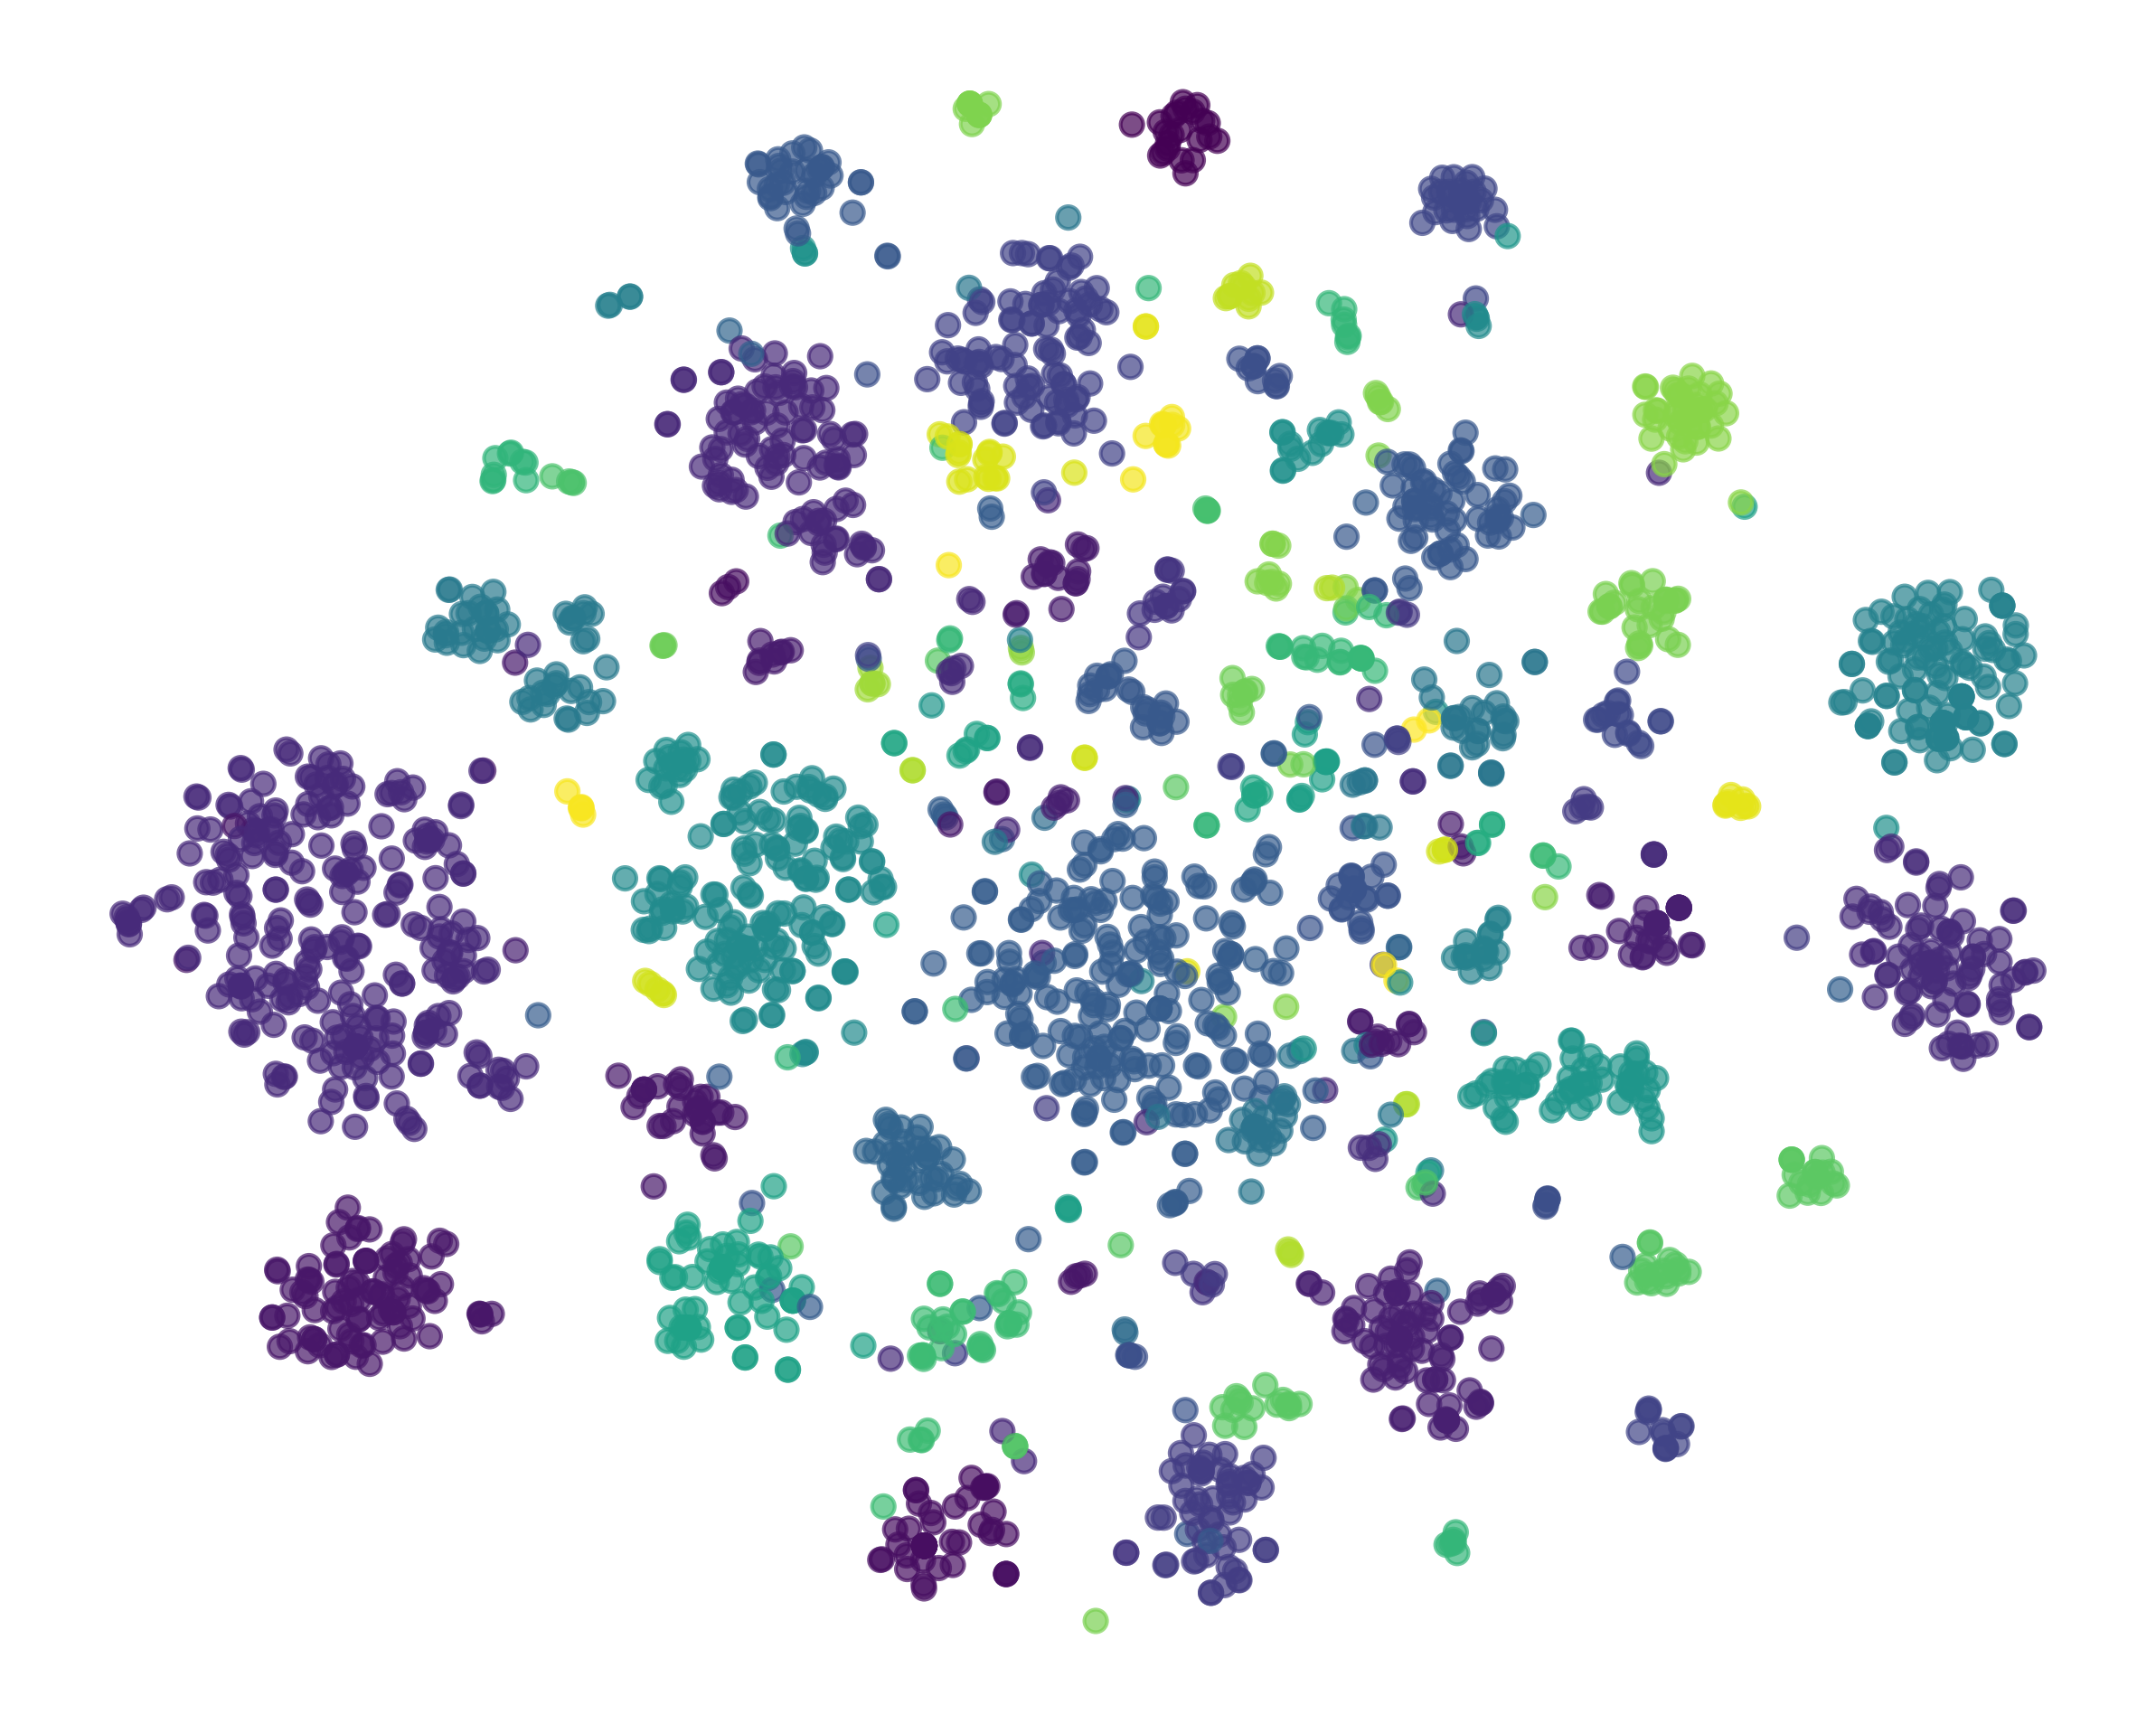
\includegraphics[width=\linewidth]{figure/Tweet_tsne.png}
        \centerline{(a) Tweet}
        \label{fig:1}
    \end{minipage}
    \hfill
    \begin{minipage}[t]{0.23\textwidth}
        \centering
        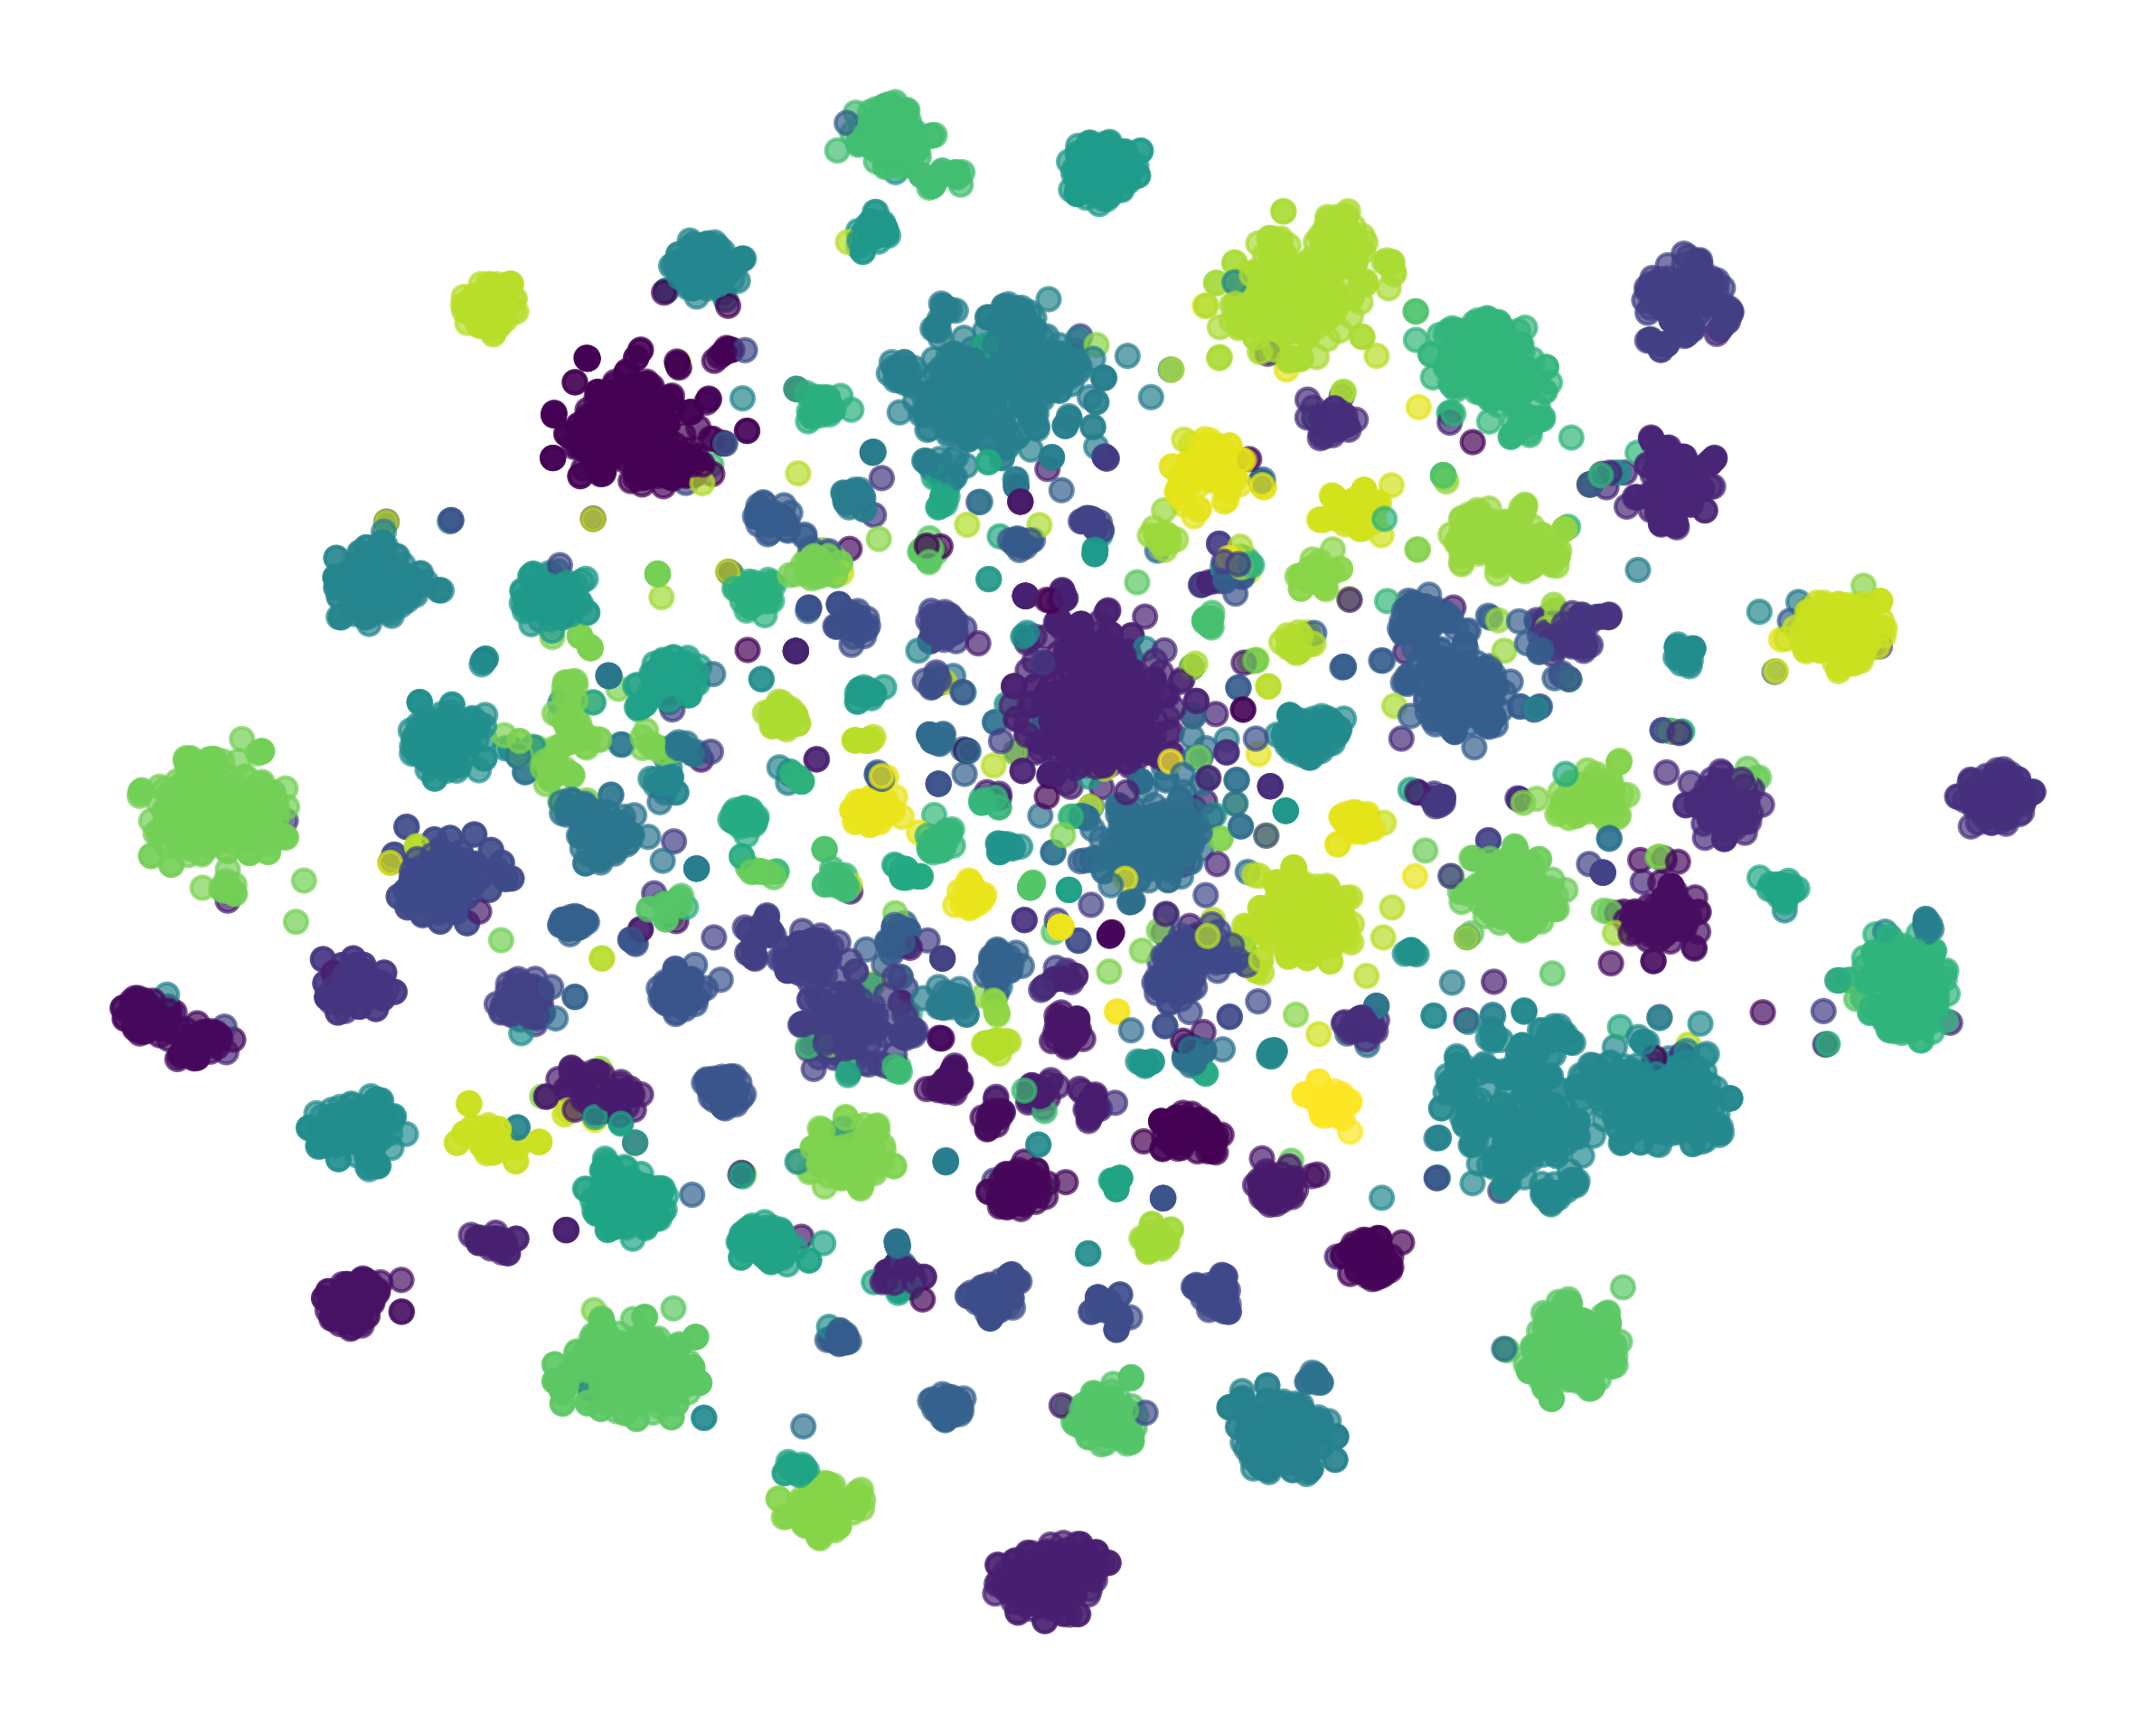
\includegraphics[width=\linewidth]{figure/S_tsne.png}
        \centerline{(b) News-S}
        \label{fig:2}
    \end{minipage}
    \hfill
    \begin{minipage}[t]{0.23\textwidth}
        \centering
        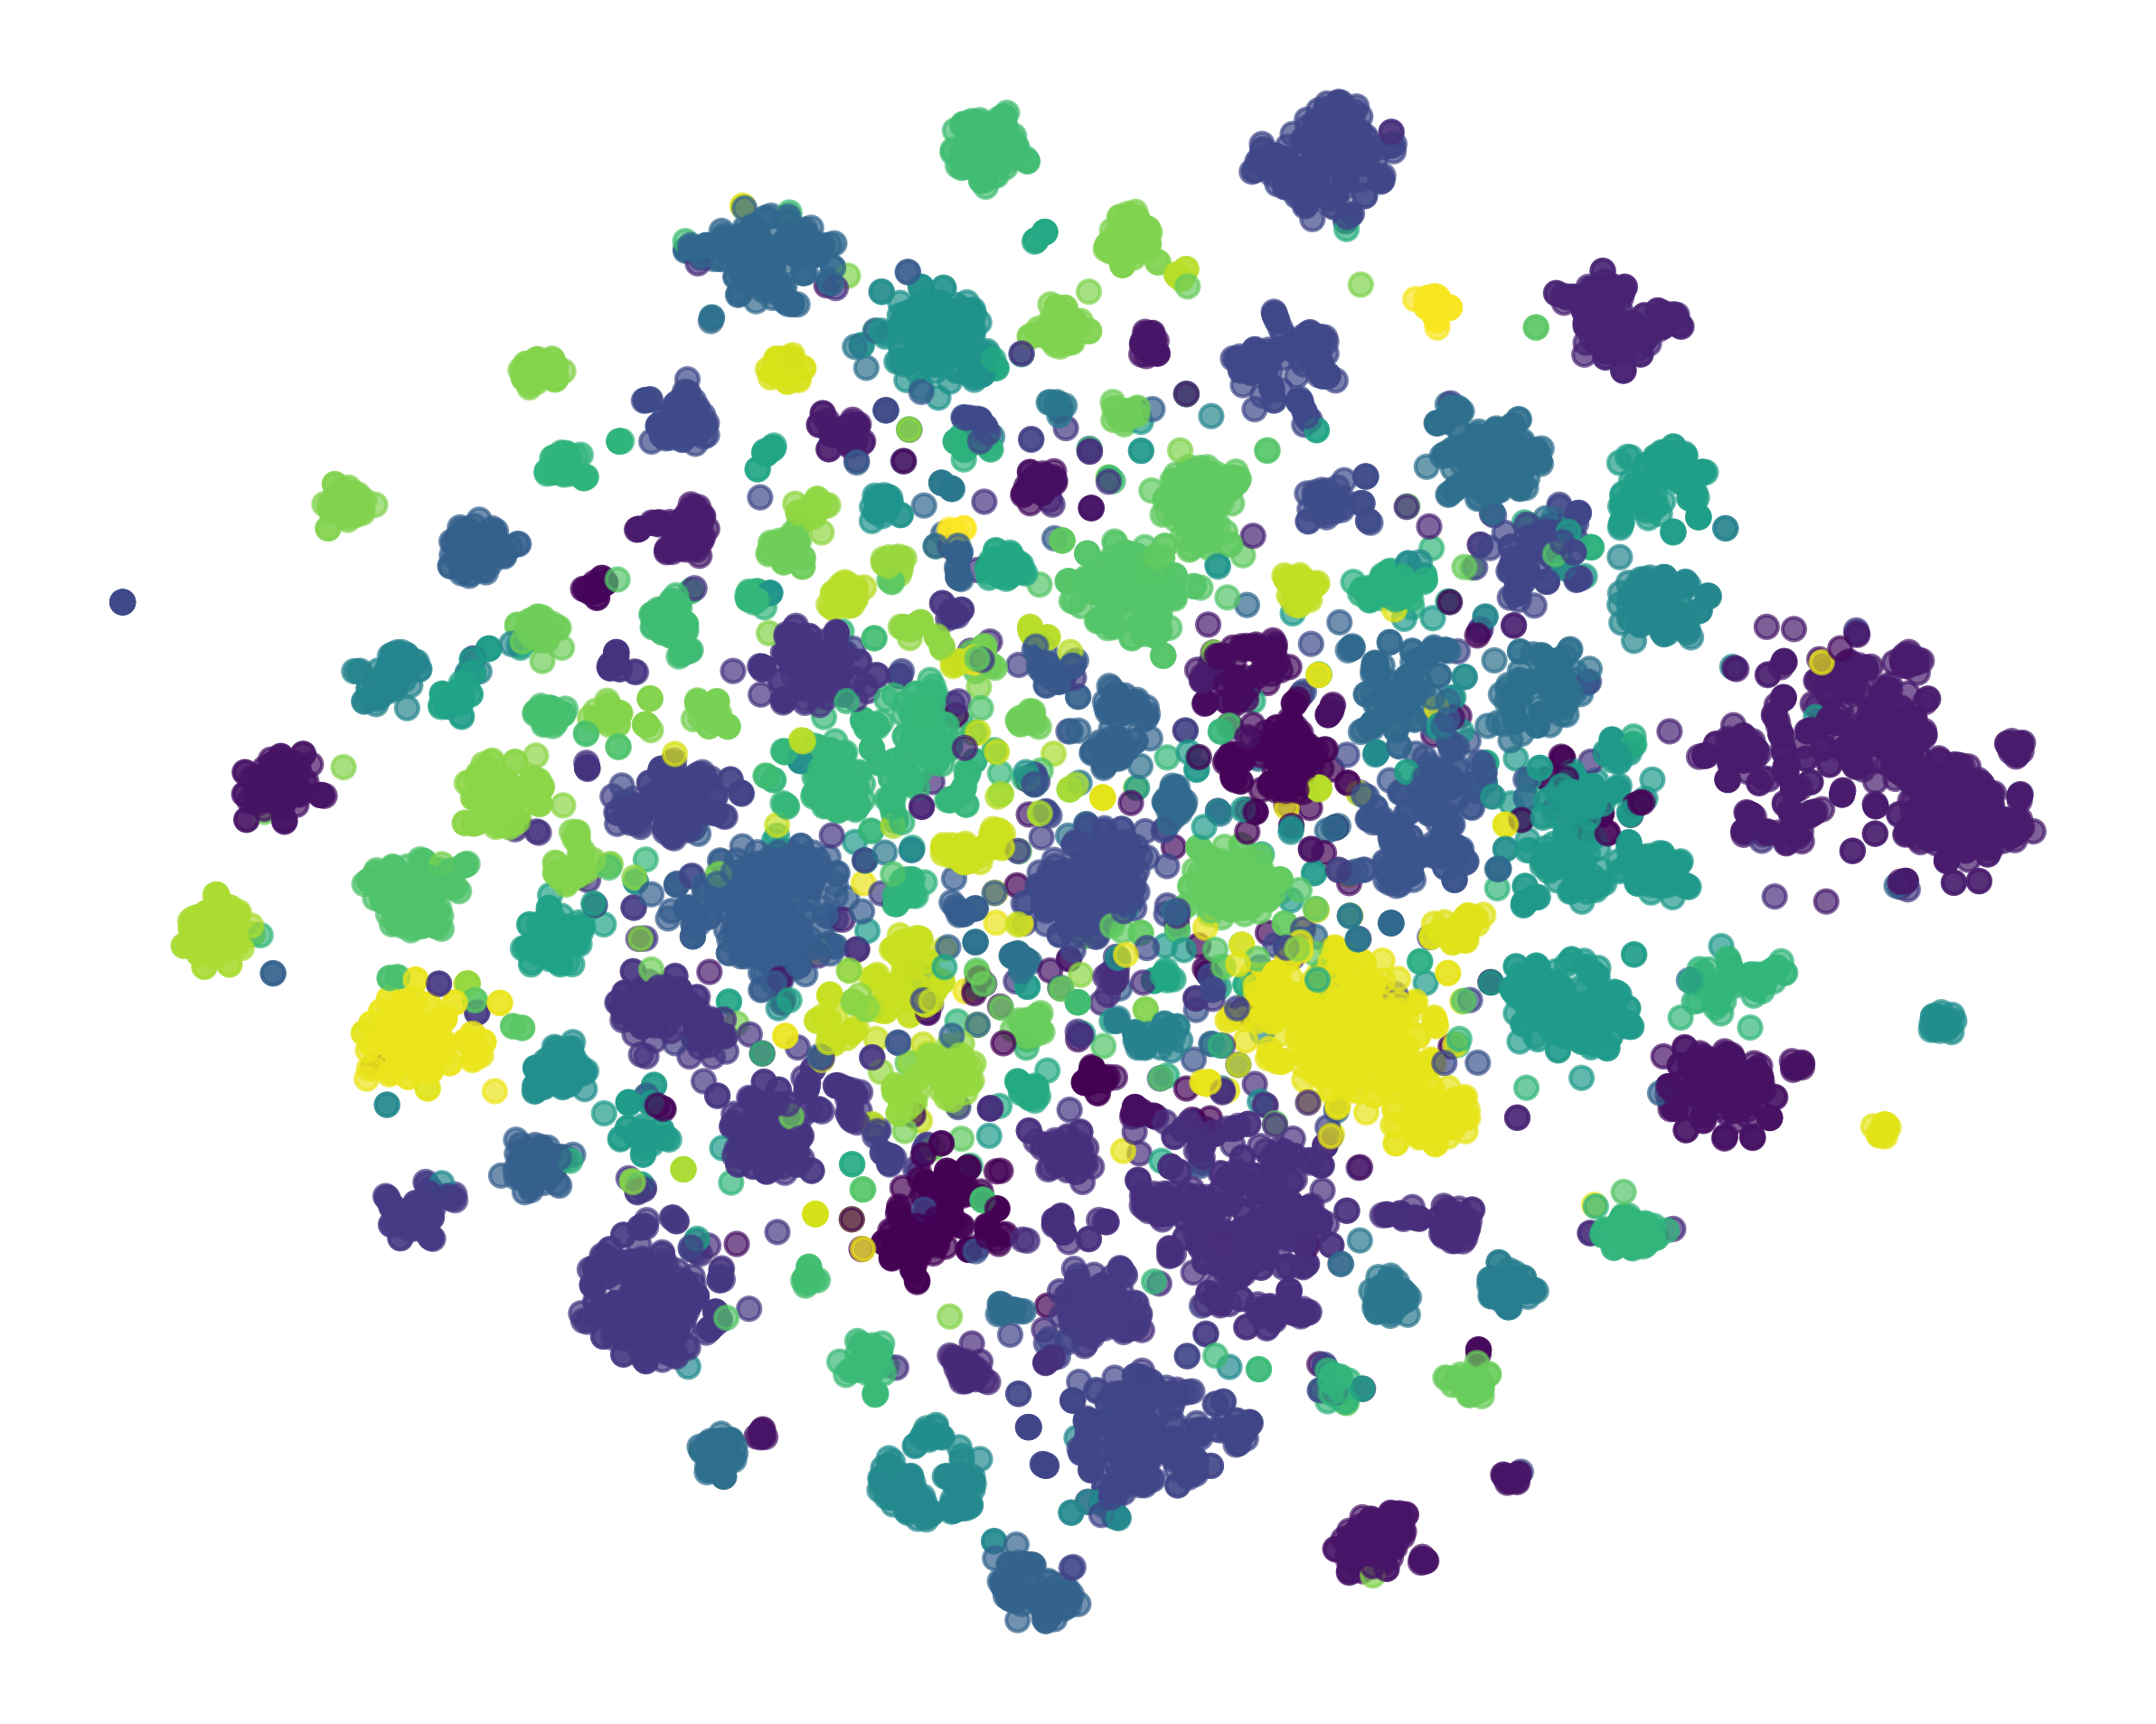
\includegraphics[width=\linewidth]{figure/T_tsne.png}
        \centerline{(c) News-T}
        \label{fig:3}
    \end{minipage}
    \hfill
    \begin{minipage}[t]{0.23\textwidth}
        \centering
        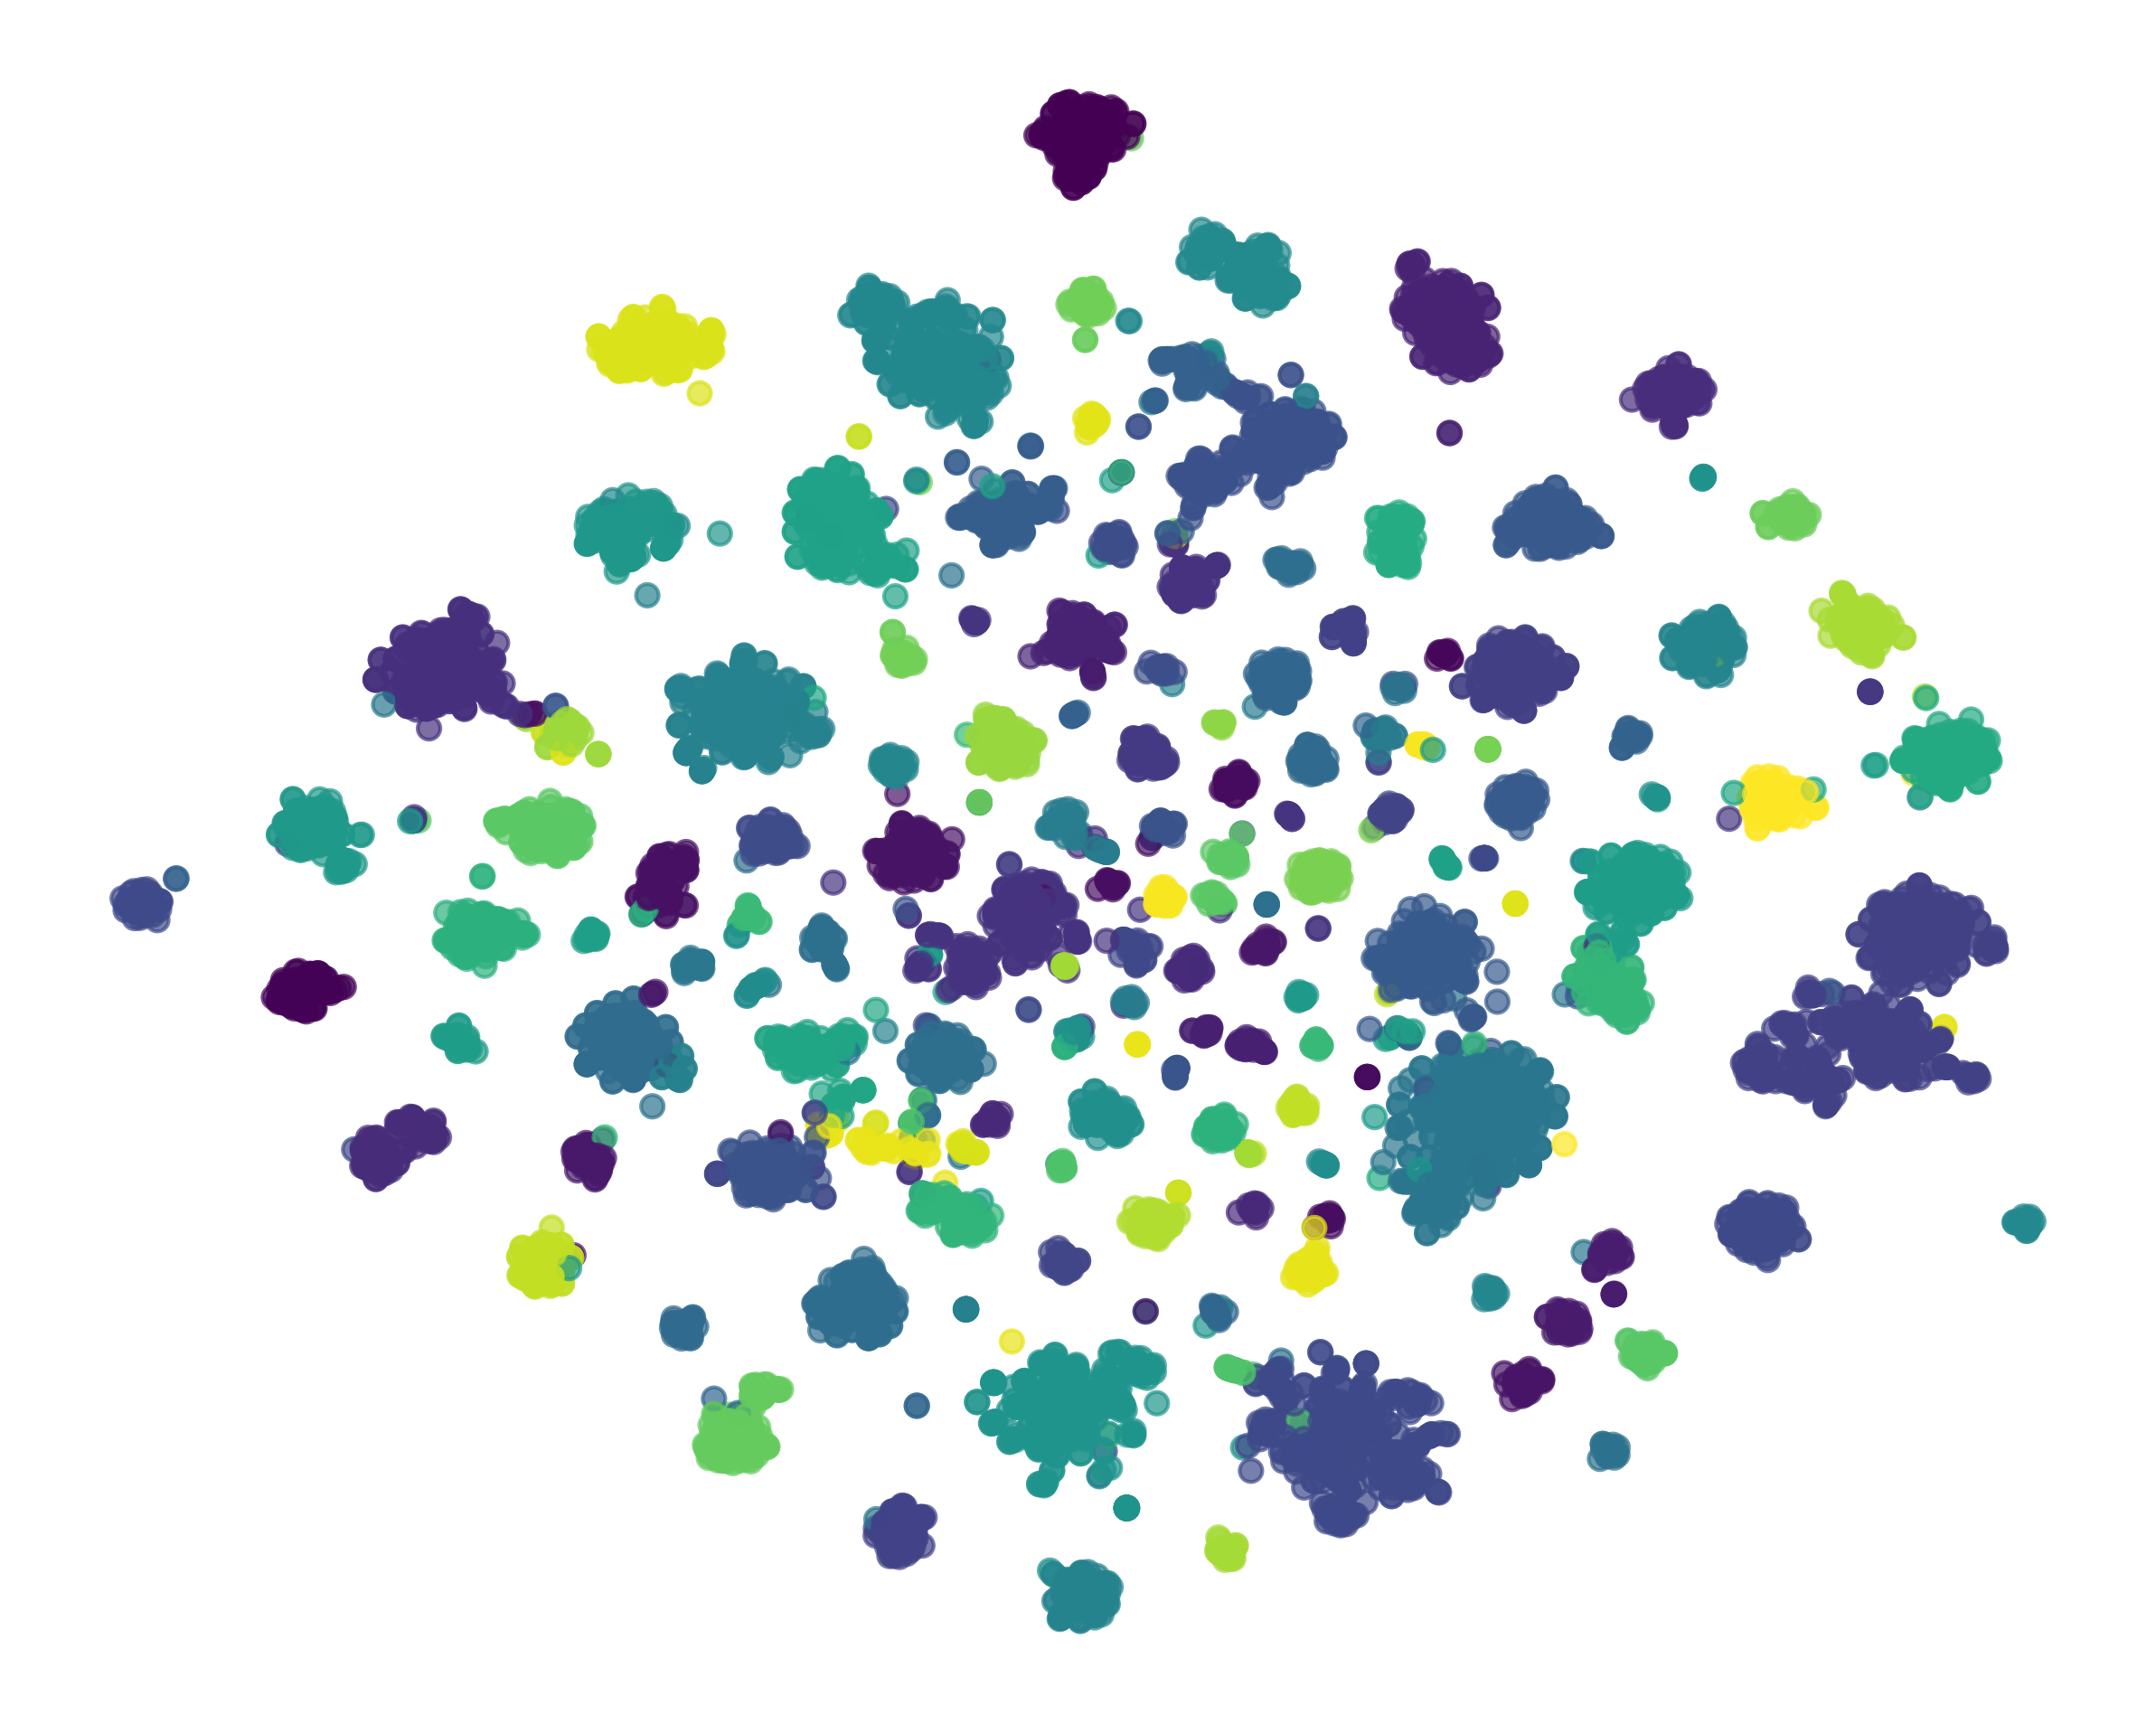
\includegraphics[width=\linewidth]{figure/TS_tsne.png}
        \centerline{(d) News-TS}
        \label{fig:4}
    \end{minipage}
\caption{2D t-SNE visualization of \sysname{} on four benchmark datasets}
\label{tsne_all}
\end{figure*}


\begin{table*}[htbp]
\centering
\renewcommand{\arraystretch}{1.2} % 调整行间距
\setlength{\tabcolsep}{7pt} % 调整列间距为12pt（默认是6pt）
\caption{The top ten representative words for the first 18 clusters discovered by \sysname{} on the News-TS dataset.}
\label{tab:clusters}
\begin{tabular}{|l|l|l|l|l|l|l|l|l|l|}
\hline
\textbf{Cluster 1} & \textbf{Cluster 2} & \textbf{Cluster 3} & \textbf{Cluster 4} & \textbf{Cluster 5} & \textbf{Cluster 6} & \textbf{Cluster} & \textbf{Cluster 8} & \textbf{Cluster 9} \\
\hline
berlusconi  & typhoon	  & google	   & illinois	 & texas	 	   & kanye	    & blackberry	 & xbox	    & hpv	 \\
vote	   & philippine	 & search	  & northern	 & nurse	 	   & west	    & bbm	         & microsoft&	vaccine	 \\
silvio	   & haiyan	     & chrome	  & lynch	     & stabbing	 	   & kim	    & android	     & console	& cancer	\\
senate	   & relief	   & voice	      & michigan	 & hospital	 	   & kardashian	 & channel	   & game	     & vaccination	\\
italian	   & aid	    & extension	    & western	 & longview	 	   & bound	    & user	      & launch	 & human	\\
italy	   & help	    & browser	    & jordan	 & center	 	   & rogen	    & device	 & playstation	& cervical	\\
rome	    & effort	 & hotword	    & husky	     & good	     	   & video	    & social	 & disc	 &papillomavirus	\\
minister	& manila	& desktop	   & game	     & tuesday	 	   & franco	    & messaging	 & user	 &gardasil	\\
government	& tacloban & hand	     & niu	         & shepherd	 	   & seth	    & app	     & drive	&study	 \\
prime	     & nov	  & free         & quarterback	 & medical	 	   & james	    & messenger	 & sony	&hea \\
\hline
\textbf{Cluster 10} & \textbf{Cluster 11} & \textbf{Cluster 12} & \textbf{Cluster 13} & \textbf{Cluster 14} & \textbf{Cluster 15} & \textbf{Cluster 16} & \textbf{Cluster 17} & \textbf{Cluster 18}\\
\hline
comet	     & lakers	    & hanukkah	     & hewlett	 & group	      	 & black	    & launch		 & chelsea	    &homefront	\\
ison	     & bryant	    & thanksgiving	 & packard	 & tax	          	 & friday	    & spacex		 & basel		& statham	\\
sun	         & kobe	        & thanksgivukkah & hp	     & political	 	 & thanksgiving	 & satellite	 & league		& jason		\\
nasa	     & los	        & year	         & earnings	 & irs	          	 & shopping	     & rocket		 & champion		&movie		\\
thanksgiving	& angeles	 & holiday	     & quarter	 & exempt	         & deal	        & falcon		 & mourinho		&action	\\
nov	       & extension	    & day	        & hpq	     & rule	             & holiday	    & commercial	 & jose		    &stallone	\\
day	       & wizard	       & jewish	        & company	 & obama	      	 & day	       & monday			 & tuesday		& review	\\
solar	   & year	       & time	        & revenue	 & proposed	      	 & store	   & attempt		 & group		& franco	\\
astronomer	 & contract	   & menorah	    & share	     & tuesday	      	 & monday	   & space		     & salah		& sylvester	\\
image	   & washin	       & turkey	        & fourth	 & administration 	 & cyber	   & cape		     & despite		& film	\\
\hline
\end{tabular}
\end{table*}

To further demonstrate the superiority of \sysname{} intuitively, we conduct 2D t-SNE~\cite{van2008visualizing} on four different datasets. Unlike previous methods that rely on model-learned embeddings and ground-truth labels to evaluate representation learning capabilities, we adopt a different approach in this section. Specifically, we use TF-IDF to obtain fixed vector representations for each text and perform t-SNE visualization in conjunction with the cluster labels obtained from our model. This approach effectively evaluates the quality of the clustering results. As shown in Figure~\ref{tsne_all}, our model successfully groups text data into distinct clusters, demonstrating its effectiveness.

Table~\ref{tab:clusters} presents the top ten representative words for the first 18 clusters discovered by \sysname{} on the News-TS dataset. Since the dataset is categorized based on events, a single representative word may not fully convey the meaning of class. However, by analyzing the representative words within each cluster, we observe that most clusters exhibit strong semantic consistency and clear event-oriented categorization, effectively capturing key information across different domains. For example, cluster 3 pertains to discussions on google search and chrome browser features, while cluster 8 focuses on gaming and console-related topics.

% 表\ref{tab:clusters} shows News-TS数据集的 top ten representative words for the 前 18 clusters found by \sysname{}. 由于数据集根据事件进行类别的划分，一个簇没有一个代表词进行表示，但是我们通过观察我们聚类结果的簇内these representative words的单词含义，例如Topic 3指向了谷歌搜索与Chrome浏览器功能的讨论，Topic 8指向游戏与主机类话题，我们可以看到绝大多数簇均具有较好的语义一致性和明确的事件指向。能够较好地捕捉不同领域的核心信息。
